\documentclass{article}
\usepackage{graphicx}
\usepackage{amsmath}
\usepackage{amssymb}
\usepackage[a4paper, top=25mm, bottom=25mm, left=25mm, right=25mm]{geometry}
\usepackage{pgfplots}
\pgfplotsset{compat=1.18}
\usepackage{mathtools}

\begin{document}
\pagestyle{empty}
\large

\begin{center}
2021-2022 Spring \\MAT124 Midterm\\(20/04/2022)
\end{center}

\noindent 1. Find the convergence set of the power series $\displaystyle\sum_{k=1}^\infty\frac{(\ln k)x^k}k$.

\hfill

\noindent 2. Show that the vectors $\mathbf{u}=\mathbf{i}+3\mathbf{j}+\mathbf{k},\:\mathbf{v}=2\mathbf{i}-\mathbf{j}-\mathbf{k}$, and $\mathbf{w}=7\mathbf{j}+3\mathbf{k}$ are coplanar (all in the same plane).

\hfill

\noindent 3. Find the point where the line

\[x-1=z,\:y=3\]

\hfill

\noindent intersects the plane $2y-z=5$.

\hfill

\noindent 4. Sketch the graphs of the following surfaces.

\hfill

\noindent (a) $z=\sin x$

\hfill

\noindent (b) $y=z^2-x^2$

\hfill

\noindent 5. Let $f$ be the function $\displaystyle f(x,y)=\frac{xy^2}{x^2+y^4}$ for $(x,y)\neq(0,0)$. Show that $f$ has no limit at $(0,0)$.

\hfill

\noindent 6. Van der Waal's equation in physical chemistry states that a gas occupying volume $V$ at temperature $T$ (Kelvin) exerts pressure $P$, where

\[\left(P+\frac A{V^2}\right)(V-B)=kT\]

\hfill

\noindent for physical constants $A, B$ and $k$. Compute the following rates.

\hfill

\noindent (a) the rate of change of volume with respect to temperature.

\hfill

\noindent (b) the rate of change of pressure with respect to volume.

\hfill

\noindent 7. Consider the surface $z=x^2+y^2-xy$, a paraboloid, on which a particle moves with $x$ and $y$ and coordinates given by $x=\cos t$ and $y=\sin t$. Using the chain rule, find $\displaystyle\frac{dz}{dt}$ when $t=0$. 

\hfill

\noindent 8. Find the parametric equations of the tangent line to the curve of intersection of the paraboloid $z=x^2+y^2$ and the ellipsoid $2x^2+2y^2+z^2=8$ at $P=(-1,1,2)$.

\newpage

\begin{center}
2021-2022 Spring Midterm (20/04/2022) Solutions\\
(Last update: 26/08/2025 23:42)
\end{center}

\noindent 1. Apply the Ratio Test for absolute convergence, and apply other tests at the endpoints.

\[\lim_{k\to\infty}\left|\frac{\ln(k+1)\cdot x^{k+1}}{k+1}\cdot\frac k{\ln(k)\cdot x^k}\right|=\lim_{k\to\infty}\left|x\cdot\frac{k}{k+1}\cdot\frac{\ln(k+1)}{\ln(k)}\right|=|x|\cdot1=|x|\]

\hfill

\noindent $k/(k+1)\to1$ and $\ln(k)/\ln(k+1)\to1$ as $k\to\infty$. Therefore, the limit is $|x|$.

\[|x|<1\implies-1<x<1\quad(\text{convergent})\]


\hfill

\noindent Investigate the convergence at the endpoints.

\[x=1\implies \sum_{k=1}^{\infty}\frac{(\ln k)\cdot 1^k}{k}=\sum_{k=1}^{\infty}\frac{\ln k}{k}\]

\hfill

\noindent Take the corresponding function $f(x)=\dfrac{\ln x}x$. The function is continuous and positive for $x>1$. It is also decreasing for $x>\mathrm{e}$ because $x$ grows faster than $\ln x$. Confirm the behavior by taking the first derivative.

\[f'(x)=\frac{1-\ln x}{x^2}<0\quad\text{for}\quad x>\mathrm e\]

\hfill

\noindent We may now apply the Integral Test.

\[\int_1^{\infty}\frac{\ln x}x\,dx=\lim_{R\to\infty}\int_1^R\frac{\ln x}x\,dx=\lim_{R\to\infty}\left.\frac12\left(\ln x\right)^2\right|_1^R=\frac12\lim_{R\to\infty}\left((\ln R)^2-(\ln1)^2\right)=\infty\]

\hfill

\noindent Since the integral diverges, by the Integral Test, the series $\displaystyle\sum_{k=1}^{\infty}\frac{\ln k}k$ also diverges. Try $x=-1$.

\[x=-1\implies \sum_{k=1}^{\infty}\frac{(\ln k)\cdot(-1)^k}{k}\]

\hfill

\noindent This is an alternating series. The non-alternating part, which is $\dfrac{\ln k}k$, is nonincreasing for $k>\mathrm{e}$ and it is positive. The previous cases are already confirmed for $x=1$. The limit at infinity is $0$. By Leibniz's Alternating Series Test, the series converges.

\hfill

\noindent Thus, the convergence set for the power series is $\boxed{[-1,1)}$.

\hfill

\noindent 2. If $\mathbf{w}\cdot(\mathbf{u}\times\mathbf{v})=0$, the vectors are coplanar. Because $\mathbf{u}\times\mathbf{v}$ is perpendicular to $\mathbf u$ and $\mathbf v$, and the resulting vector is also perpendicular to $\mathbf w$. Compute the cross product.

\begin{align*}\mathbf{u}\times\mathbf{v}&=\left|\begin{array}{ccc}
\mathbf{i}&\mathbf{j}&\mathbf{k}\\
1&3&1\\
2&-1&-1
\end{array}\right|=\mathbf{i}\left|\begin{array}{cc}
3&1\\-1&-1
\end{array}\right|-\mathbf{j}\left|\begin{array}{cc}
1&1\\2&-1
\end{array}\right|+\mathbf{k}\left|\begin{array}{cc}
1&3\\2&-1
\end{array}\right|\\\\&=(-1\cdot3-1\cdot(-1))\mathbf{i}-(-1\cdot1-2\cdot1)\mathbf{j}+(-1\cdot1-3\cdot2)\mathbf{k}=-2\mathbf i+3\mathbf j-7\mathbf k\end{align*}

\hfill

\noindent Compute the dot product.

\[\mathbf w\cdot(\mathbf u\times\mathbf v)=(7\mathbf j+3\mathbf k)\cdot(2\mathbf i+3\mathbf j-7\mathbf k)=0\cdot2+7\cdot3+3\cdot(-7)=0\]

\hfill

\noindent Therefore, all the vectors are coplanar.

\hfill

\noindent 3. For $y=3$, $2y-z=5\implies6-z=5\implies z=1$. For $z=1$, $x-1=z\implies x-1=1\implies x=2$. Therefore, the point where the line and the plane intersect is $\boxed{(2,3,1)}$.

\hfill

\noindent 4.

\hfill

\noindent (a)
\begin{center}
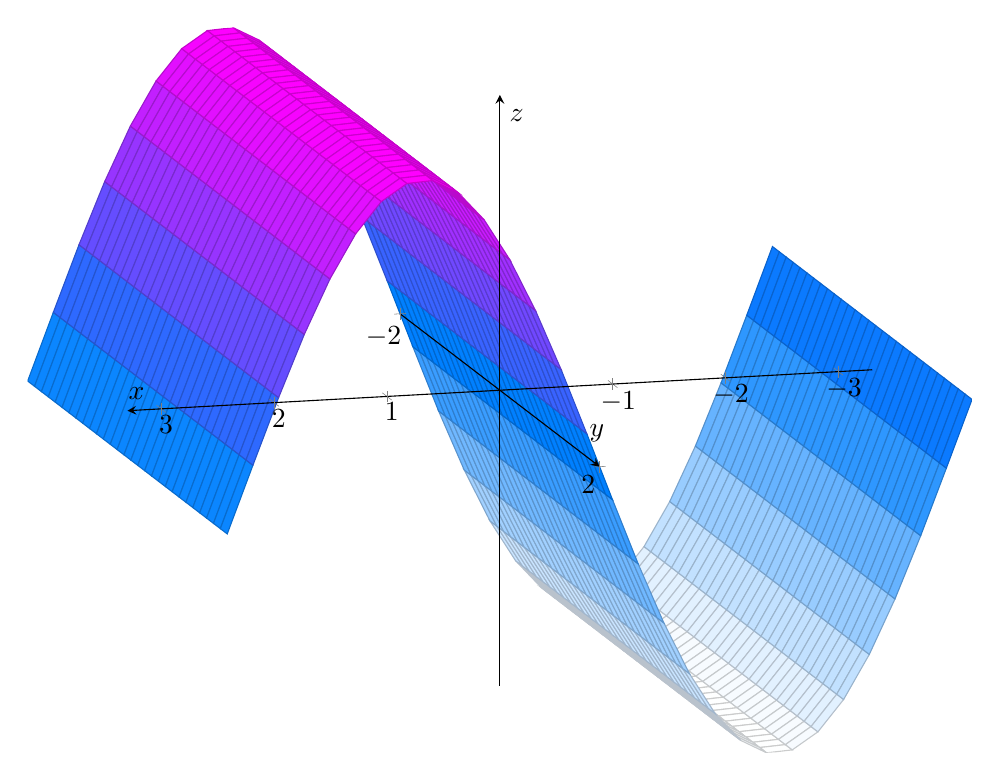
\begin{tikzpicture}
  \begin{axis}[
    view={165}{15},
    axis lines=center,
    xlabel={$x$},
    ylabel={$y$},
    zlabel={$z$},
    domain=-3.3:3.3,
    y domain=-2:2,
    samples=30,
    samples y=30,
    colormap/cool,
    z buffer=sort,
    axis on top,
    scale=1.75,
    ztick={-1,1}
  ]
    \addplot3[surf] {sin(deg(x)};
    \end{axis}
\end{tikzpicture}
\end{center}

\newpage

\noindent (b)
\begin{center}
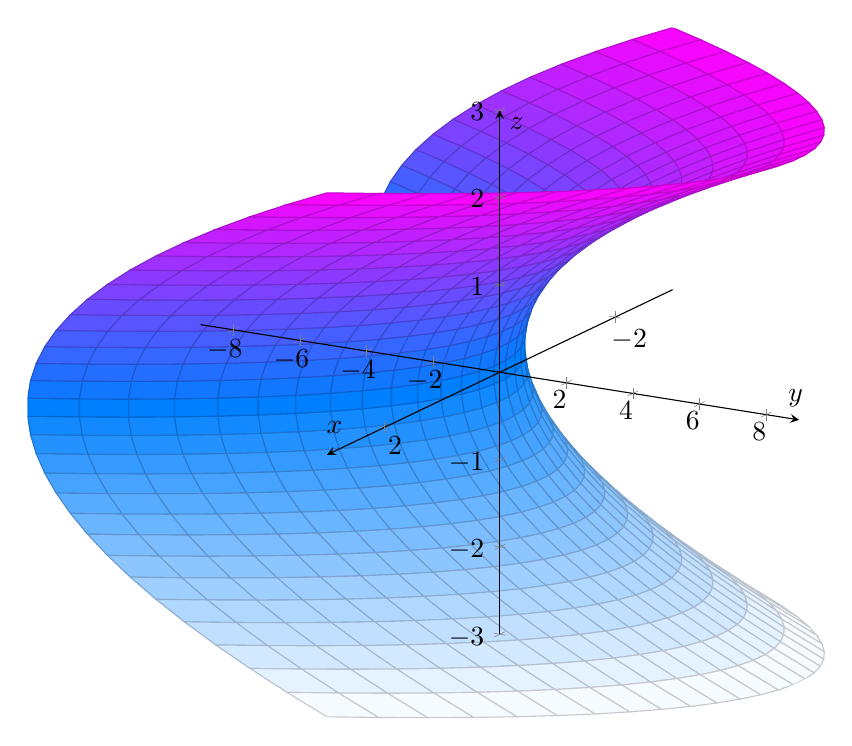
\begin{tikzpicture}
  \begin{axis}[
    view={120}{20},
    axis lines=center,
    xlabel={$x$},
    ylabel={$y$},
    zlabel={$z$},
    domain=-3:3,
    y domain=-3:3,
    samples=30,
    samples y=30,
    colormap/cool,
    z buffer=sort,
    axis on top,
    scale=1.75
  ]
    \addplot3[surf]({x}, {y^2 - x^2}, {y});
  \end{axis}
\end{tikzpicture}
\end{center}

\hfill

\noindent 5. Apply the Two-Path Test.

\[y=x\implies\lim_{(x,y)\to(0,0)}\frac{xy^2}{x^2+y^4}=\lim_{x\to0}\frac{x^3}{x^2+x^4}=\lim_{x\to0}\frac{x}{1+x^2}=\frac01=0\]
\[x=y^2\implies\lim_{(x,y)\to(0,0)}\frac{xy^2}{x^2+y^4}=\lim_{y\to0}\frac{y^4}{2y^4}=\frac12\]

\hfill

\noindent Since $0\neq\dfrac12$, by the Two-Path Test, the limit does not exist.

\hfill

\noindent 6.

\hfill

\noindent (a) Apply the product rule.

\[\frac\partial{\partial T}\left[\left(P+\frac A{V^2}\right)(V-B)\right]=\frac\partial{\partial T}\left(kT\right)\]

\[\left(\frac{\partial P}{\partial T}-\frac{2A}{V^3}\cdot\frac{\partial V}{\partial T}\right)(V-B)+\left(P+\frac A{V^2}\right)\left(\frac{\partial V}{\partial T}\right)=k\]

\[(V-B)\frac{\partial P}{\partial T}+\frac{\partial V}{\partial T}\left(-\frac{2A}{V^2}+\frac{2AB}{V^3}\right)+\frac{\partial V}{\partial T}\left(P+\frac{A}{V^2}\right)=k\]

\[\boxed{\frac{\partial V}{\partial T}=\frac{k+(B-V)\dfrac{\partial P}{\partial T}}{P+\dfrac{2AB}{V^3}-\dfrac{A}{V^2}}}\]

\hfill

\noindent (b) Apply the product rule again.

\[\frac\partial{\partial V}\left[\left(P+\frac A{V^2}\right)(V-B)\right]=\frac\partial{\partial V}\left(kT\right)\]

\[\left(\frac{\partial P}{\partial V}-\frac{2A}{V^3}\right)(V-B)+\left(P+\frac A{V^2}\right)\cdot1=k\frac{\partial T}{\partial V}\]

\[(V-B)\frac{\partial P}{\partial V}-\frac{2A}{V^2}+\frac{2AB}{V^3}=k\frac{\partial T}{\partial V}-P-\frac A{V^2}\]

\[\boxed{\frac{\partial P}{\partial V}=\frac{k\dfrac{\partial T}{\partial V}-P+\dfrac A{V^2}-\dfrac{2AB}{V^3}}{V-B}}\]

\hfill

\noindent 7. $z=z(x,y),\:x=x(t)$ and $y=y(t)$. Apply the chain rule.

\begin{align*}\frac{dz}{dt}&=\frac{\partial z}{\partial x}\cdot\frac{dx}{dt}+\frac{\partial z}{\partial y}\cdot\frac{dy}{dt}=(2x-y)(-\sin t)+(2y-x)(\cos t)\\\\&=(2\cos t-\sin t)(-\sin t)+(2\sin t-\cos t)(\cos t)=\sin^2t-\cos^2t=-\cos2t\end{align*}

\hfill

\noindent The result is then

\[\left.\frac{dz}{dt}\right|_{t=0}=-\cos0=\boxed{-1}\]

\hfill

\noindent 8. Let $f(x,y,z)=x^2+y^2-z=0$ and $g(x,y,z)=2x^2+2y^2+z^2=8$ be level surfaces. The tangent line is perpendicular to both $\nabla f$ and $\nabla g$ at $P$.

\[\nabla f=\left\langle2x,2y,-1\right\rangle,\qquad\nabla g=\left\langle4x,4y,2z\right\rangle\]
\[\nabla f(P)=\left\langle-2,2,-1\right\rangle,\qquad\nabla g(P)=\left\langle-4,4,4\right\rangle\]

\begin{align*}\mathbf{T}&=\nabla f\times\nabla g=\left|\begin{array}{ccc}
\mathbf{i}&\mathbf{j}&\mathbf{k}\\
-2&2&-1\\
-4&4&4
\end{array}\right|=\mathbf{i}\left|\begin{array}{cc}
2&-1\\4&4
\end{array}\right|-\mathbf{j}\left|\begin{array}{cc}
-2&-1\\-4&4
\end{array}\right|+\mathbf{k}\left|\begin{array}{cc}
-2&2\\-4&4
\end{array}\right|\\\\&=(2\cdot4-4\cdot(-1))\mathbf{i}-(-2\cdot4-(-4)\cdot(-1))\mathbf{j}+(-2\cdot4-2\cdot(-4))\mathbf{k}=12\mathbf i+12\mathbf j\end{align*}

\hfill

\noindent The parametric equations for the tangent line is

\[\boxed{\left.\begin{array}{l}
x=-1+12t\\
y=1+12t\\
z=2
\end{array}\right\}\quad t\in\mathbb{R}}\]

\end{document}